\label{sec:chap5}
\section{簡介}
在前一章節,利用專注式機制學習較好的向量表示,成功將平均準確率大幅提升。在本章中,想引入語音詞向量(Audio
Word2vec)的概念,在語音詞向量模型中,會先將語音文件依照文字的邊界切斷,但要如此做必須先切出文字邊界,才能產生出語音詞向量。在本章中,將不切出文字邊界而是直接產生出代表查詢詞跟語音文字的向量表示,並藉由分類器判斷語音文件是否出現查詢詞。
\section{語音詞向量}
語音詞向量的概念為詞向量(Word Vector)的延伸,詞向量又稱詞嵌入(Word
Embedding)能夠將詞轉成有意義的向量。詞嵌入表示能夠將語意關係或句法結構的關係,用兩個向量之間的歐式距離(Euclidean
Distance)或餘弦相似度(Cosine
Similarity)之大小就能呈現出來,例如母親與父親的歐式距離跟國王與皇后的歐式距離是相差不遠的。語音詞向量則是希望在語音輸入下,也能夠有如此的效果。
\begin{figure}[h]
\centering
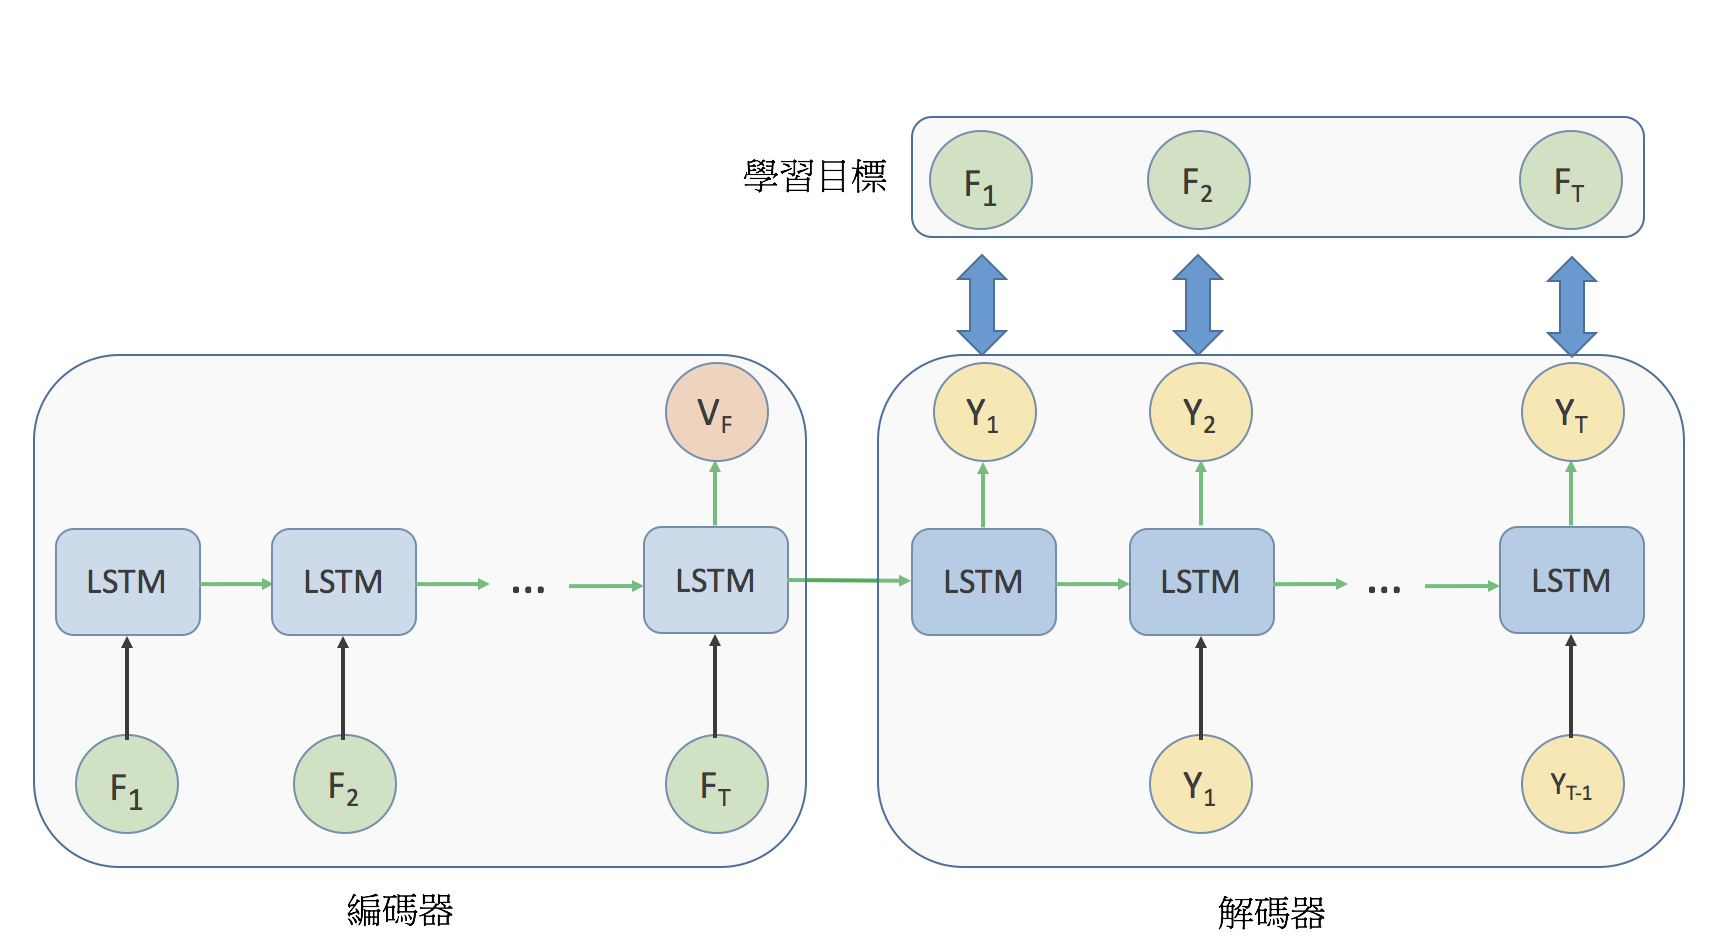
\includegraphics[scale=0.5]{images/ch5_seq2seq.png} 
\caption{語音詞向量模型圖}
\label{ch5_seq2seq}
\end{figure}
\label{ch5_seq2seq}
圖\ref{ch5_seq2seq}為語音詞向量的模型架構
\section{模型架構}
\section{實驗與分析}
\section{本章總結}
